\documentclass[12pt]{article}
\usepackage[english]{babel}
\usepackage[utf8]{inputenc} % Permite el uso de caracteres del Español
\usepackage[T1]{fontenc}
\usepackage{graphicx}
\usepackage{amsmath}
\usepackage{wrapfig}
\usepackage{enumerate}
\usepackage[top=1in, bottom=1.25in, left=1.1in, right=1.1in]{geometry}
\usepackage[dvipsnames]{xcolor}
\usepackage{subcaption}

\begin{document}

\begin{titlepage}

\newcommand{\HRule}{\rule{\linewidth}{0.5mm}} % Define un comando para las lineas horizontales

\center 
%----------------------------------------------------------------------------------------
%	Cabezera
%----------------------------------------------------------------------------------------

\textsc{\LARGE Universidad de Sonora}\\[1.5cm]
\textsc{\Large Licenciatura en Física}\\[0.5cm]
\textsc{\large Física Computacional I}\\[0.5cm]

%----------------------------------------------------------------------------------------
%	Titulo
%----------------------------------------------------------------------------------------

\HRule \\[0.4cm]
{\huge \bfseries Actividad 6 - Sistema de resortes acoplados}\\[0.4cm] % Title of your document
\HRule \\[1.5cm]
 
%----------------------------------------------------------------------------------------
%	Autor
%----------------------------------------------------------------------------------------

\begin{minipage}{0.4\textwidth}
\begin{flushleft} \large
\emph{Alumno:}\\
José Gabriel Navarro I.
\end{flushleft}
\end{minipage}
~
\begin{minipage}{0.4\textwidth}
\begin{flushright} \large
\emph{Profesor:} \\
Carlos Lizarraga Celaya
\end{flushright}
\end{minipage}\\[2cm]


%----------------------------------------------------------------------------------------
%	Fecha
%----------------------------------------------------------------------------------------
15 de Marzo de 2018

%----------------------------------------------------------------------------------------
%	Escudo
%----------------------------------------------------------------------------------------


\includegraphics[width=0.4\textwidth]{logo.png}\\
 
%----------------------------------------------------------------------------------------

\vfill % Llena el espacio de la pagina en blanco

\end{titlepage}

\section{Introducción}
En el presente reporte se habla acerca de la sexta actividad realizada para la clase de Física Computacional I, el cual abarca el análisis de las ecuaciones de un sistema de resortes acoplados. \\

Primeramente se muestra una síntesis acerca de la teoría detrás de este sistema, esto basado en el artículo "Coupled Spring Equations" de Fay y Graham. En esta misma síntesis se incluye el código utilizado en Python con la nueva herramienta de Jupyter: Jupyter Lab, para resolver estos problemas de una manera numérica. Después de esto, se presenta el error relativo que existe entre el valor numérico que se encontró utilizando la librería scipy.integrate.odeint y la solución analítica dada por el artículo.    Al final se presenta una conclusión de la actividad, así como la bibliografía utilizada para la investigación de los fundamentos y el apéndice. 

\section{Síntesis - Sistema de resortes acoplados}

\subsection{Introducción}

\begin{wrapfigure}{r}{0.2\textwidth}
    \centering
    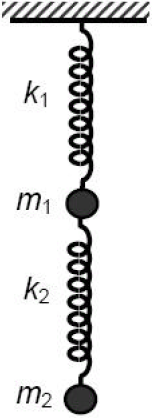
\includegraphics[width=0.1\textwidth]{ResorteAcoplado.png}
\end{wrapfigure}

En este artículo, se investiga uno de los problemas más interesantes de Mecánica, y que ahora normalmente se utiliza para la introducción al estudio de ecuaciones diferenciales. Este problema es el de dos resortes con dos masas puestas en serie, colgando del techo. Si suponemos que las fuerzas restauradoras de los resortes se comportan según la Ley de Hooke, estos dos grados de libertad nos dan un modelo de ecuaciones diferenciales lineales de segundo grado. Al sustituir una ecuación en la otra, el movimiento de las masas puede ser descrito por una ecuación diferencial lineal de cuarto grado.\\

Con estas ecuaciones, podemos investigar los movimientos de las dos masas, para saber si estas están sincronizadas (es decir en fase), o si son opuestas (en desfase). Además, también se puede observar gráficamente la periodicidad, la amplitud, la fase, y otros conceptos al modificar los parámetros de este modelo. 

\subsection{El modelo de los resortes acoplados}
Como se menciono anteriormente, el modelo consiste de dos resortes y dos masas. Un resorte, con una constante $k_1$, esta colgado del techo con una masa $m_1$ colgando de ella. De aquí, cuelga otro resorte con una constante de $k_2$ y debajo de ella cuelga una masa $m_2$.  Al dejarlo en reposo, los resortes se estiran una distancia, a la que llamaremos: $x_1$ y $x_2$. \\

\subsubsection{Asumiendo la Ley de Hooke}
Si asumimos que el sistema se mueve con oscilaciones pequeñas, podemos asumir que los resortes tendrán una fuerza restauradora dada por la Ley de Hooke, dada de la forma: $-k_1l_1$ y $-k_2l_2$ en donde $l_1$ y $l_2$ son las elongaciones o comprensiones de los dos resortes. Como $m_1$ esta atada a los dos resortes, en esta actuan las dos fuerzas restauradoras, mientras que $m_2$ solamente "siente" la fuerza restauradora del segundo resorte. Sin fricción, la segunda ley de Newton para estas dos masas son de la siguiente forma: \\

\centerline{$m_1 \ddot x_1 = -k_1x_1 - k_2(x_1-x_2)$}
\centerline{$m_2 \ddot x_2 = -k_2(x_2-x_1)$}
$    $

Para encontrar una ecuación para $x_1$ que no involucre a $x_2$, resolvermos la ecuación de $x_2$, y sustituyendo esta ecuación en las ecuaciones anteriores llegamos a la siguiente ecuación diferencial de cuarto grado: \\

\centerline{$m_1m_2x_1^{(4)} + (m_2k_1 + k_2(m_1+m_2)) \ddot x_1 + k_1k_2x_1=0$}
$    $

Y si se hace ese mismo proceso pero para $x_2$, se llega a la misma ecuación anterior. Solamente las posiciones y velocidades iniciales se necesitan para poder determinar la solución. 

\subsubsection{Algunos ejemplos con masas idénticas}
\noindent \textit{2.1 Describe el movimiento para un sistema de resortes con $k_1=6$ y $k_2=4$ con condiciones iniciales de $(x_1(0), \dot x_1(0), x_2(0), \dot x_2(0)$)=$(1,0,2,0)$.}\\

Resolviendo el problema de una forma analítica, podemos llegar a que las ecuaciones para las posiciones de las masas son: \\

\centerline{$x_1(t) = cos \sqrt 2 t$}
\centerline{$x_2(t) = 2 cos \sqrt 2 t$}
$ $

El movimiento esta sincronizado, y por lo tanto las masas se mueven en fase una con la otra. Solamente tienen amplitud diferentes. El retrato de fase de estas son elipses, y como solamente varían en amplitud, al graficar sus posiciones una contra otra, se obtiene una linea recta. A continuación se presenta el código utilizado para encontrar numéricamente estos resultados y las graficas correspondientes: \\ 

Para graficar los datos, solamente se utilizo la linea de código de lectura de datos: \textit{t, x1, xy, x2, y2, er1, er2 = loadtxt('dosresortes2\_1.dat', unpack=True)}, y se graficaron los datos como ya se ha echo anteriormente en otras practicas. \\ \\  

\begin{figure}[h!]
    \centering
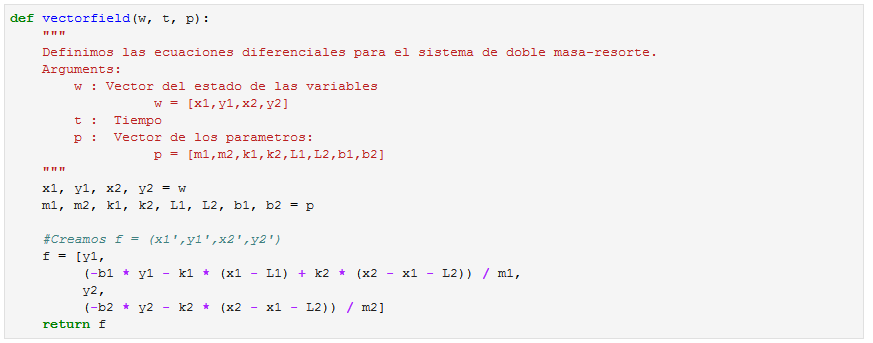
\includegraphics[width=6in]{Cod1.png}
\end{figure}

\begin{figure}[h!]
    \centering
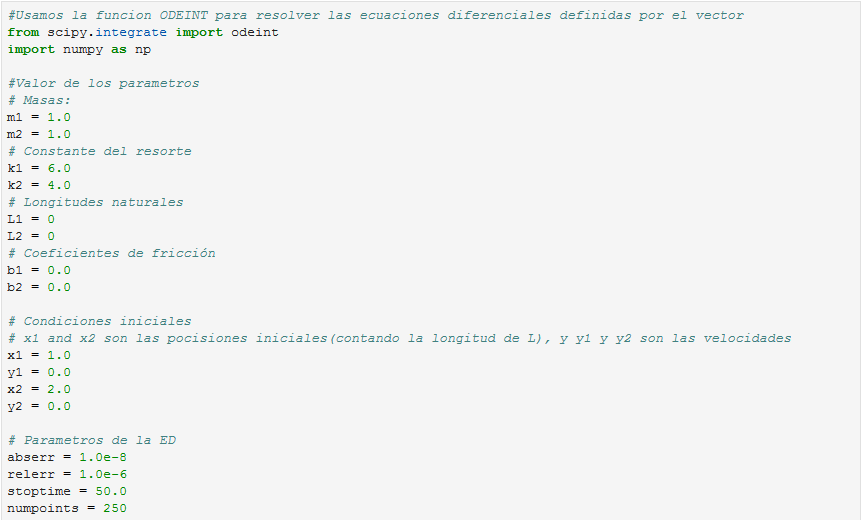
\includegraphics[width=6in]{Cod2.png}
\end{figure}

\begin{figure}[h!]
    \centering
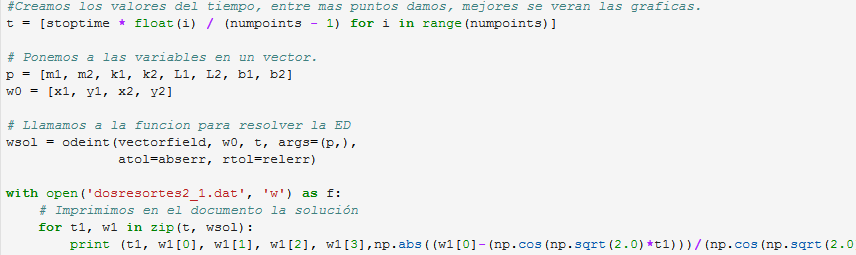
\includegraphics[width=6in]{Cod3.png}
\end{figure}

\clearpage

\begin{figure}[h!]
    \centering
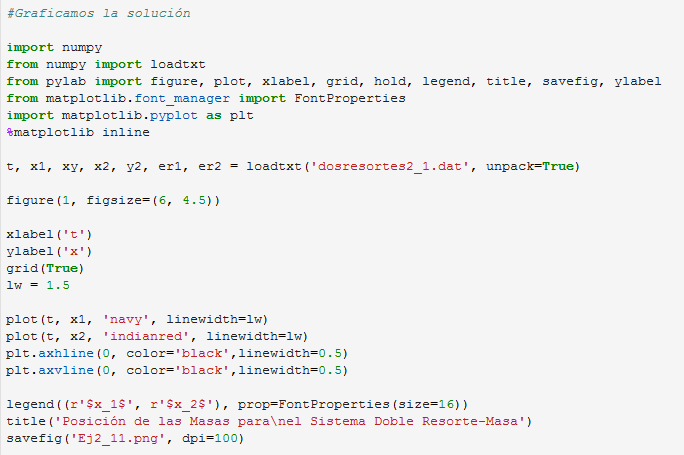
\includegraphics[width=6in]{Cod4.png}
\end{figure}

Las gráficas obtenidas son:
\begin{figure}[h!]
    \centering
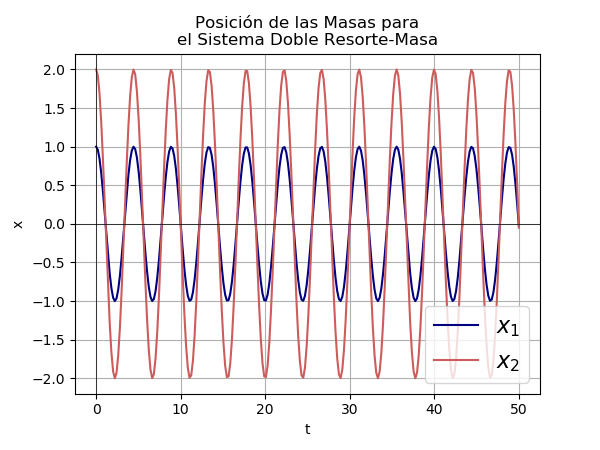
\includegraphics[width=5in]{Ej2_11.png}
\caption{Graficas de $x_1$ y $x_2$}
\end{figure}
\begin{figure}[h!]
\begin{subfigure}{.55\textwidth}
  \centering
  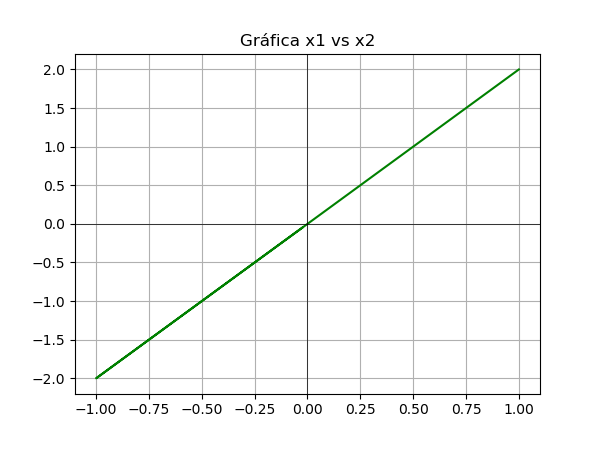
\includegraphics[width=.8\linewidth]{Ej2_12.png}
  \caption{$x_1$ vs $x_2$}
  \label{fig:sfig2}
\end{subfigure}
\begin{subfigure}{.55\textwidth}
  \centering
  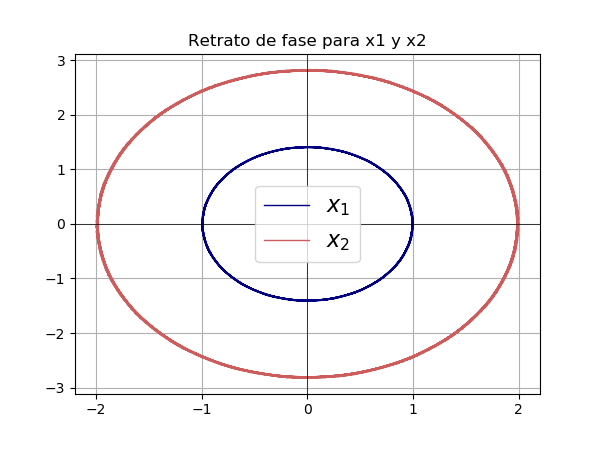
\includegraphics[width=.8\linewidth]{Ej2_13.png}
  \caption{Retrato de fase de $x_1$ y $x_2$}
  \label{fig:sfig2}
\end{subfigure}
\end{figure}

\noindent \textit{2.2 Describe el movimiento para un sistema de resortes con $k_1=6$ y $k_2=4$ con condiciones iniciales de $(x_1(0), \dot x_1(0), x_2(0), \dot x_2(0)$)=$(-2,0,1,0)$.}\\

Para este caso, la primera masa se mueve hacia abajo mientras que la otra se mueve hacia arriba, tienen el mismo periodo, pero estan fuera de fase. La solución analítica es: \\

\centerline{$x_1(t) = -2 cos 2\sqrt 3 t$}
\centerline{$x_2(t) = cos 2\sqrt 3 t$}
$ $

El código utilizado para este caso, es el mismo que se uso en el ejemplo anterior, y así fue con todos los ejemplos. Lo único que cambiaba eran los datos a utilizar y las graficas resultantes: 

\begin{figure}[h!]
    \centering
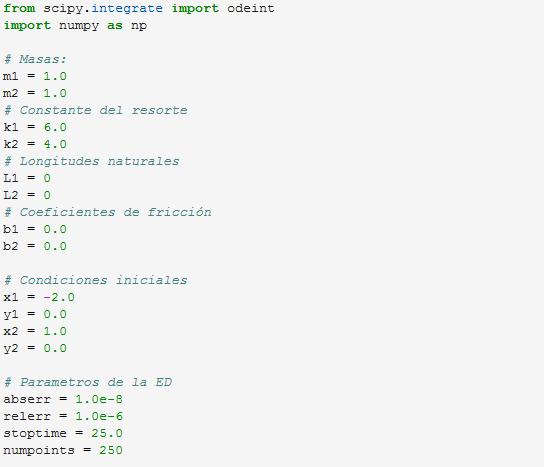
\includegraphics[width=3.5in]{Cod5.png}
\end{figure}

Las gráficas son:

\begin{figure}[h!]
\begin{subfigure}{.6\textwidth}
  \centering
  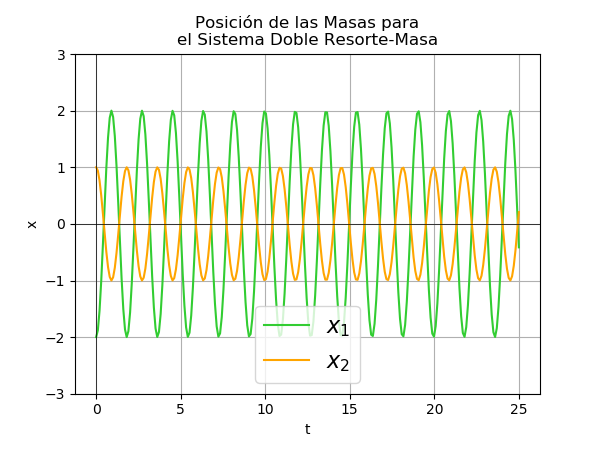
\includegraphics[width=.8\linewidth]{Ej2_21.png}
  \caption{Gráfica de $x_1$ y $x_2$}
  \label{fig:sfig2}
\end{subfigure}
\begin{subfigure}{.6\textwidth}
  \centering
  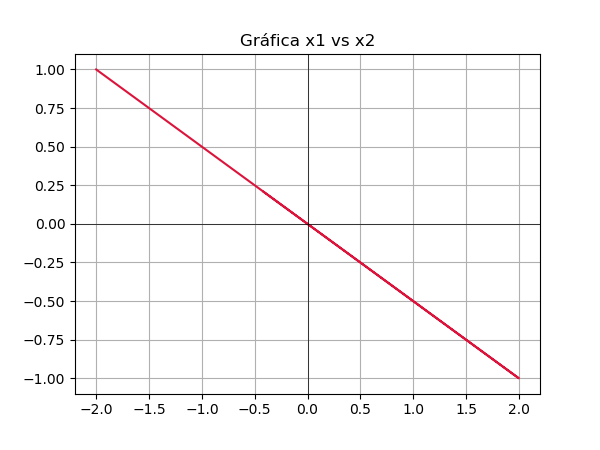
\includegraphics[width=.8\linewidth]{Ej2_22.png}
  \caption{Gráfica de $x_1$ vs $x_2$}
  \label{fig:sfig2}
\end{subfigure}
\end{figure}

\noindent \textit{2.3 Describe el movimiento para un sistema de resortes con $k_1=0.4$ y $k_2=1.808$ con condiciones iniciales de $(x_1(0), \dot x_1(0), x_2(0), \dot x_2(0)$)=$(1/2,0,-1/2,7/10)$.}\\

Con este ejemplo podemos observar como las condiciones iniciales solo afectan a la amplitud y fase de la soluciones, mientras que las constantes de los resortes determinan el periodo y frecuencia del fenómeno. Los retratos de fase son casi un movimiento periódico entre ellos, y si graficamos $x_1$ vs $x_2$ parece una curva de tipo Lissajous. En el código solamente se edito los datos como las constantes y las condiciones iniciales:

\begin{figure}[h!]
    \centering
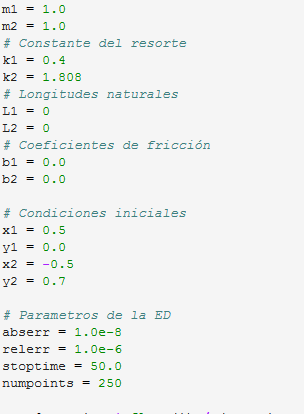
\includegraphics[width=3in]{Cod6.png}
\end{figure}

Las graficas resultantes fueron: \\ \\

\begin{figure}[h!]
\begin{subfigure}{.55\textwidth}
  \centering
  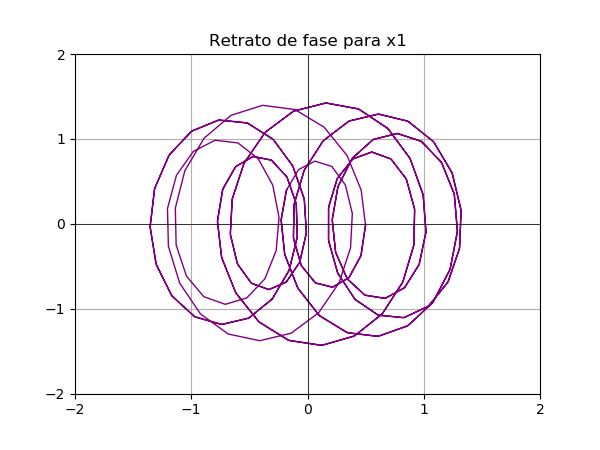
\includegraphics[width=.8\linewidth]{Ej2_31.png}
  \caption{Retrato de fase de $x_1$}
  \label{fig:sfig2}
\end{subfigure}
\begin{subfigure}{.55\textwidth}
  \centering
  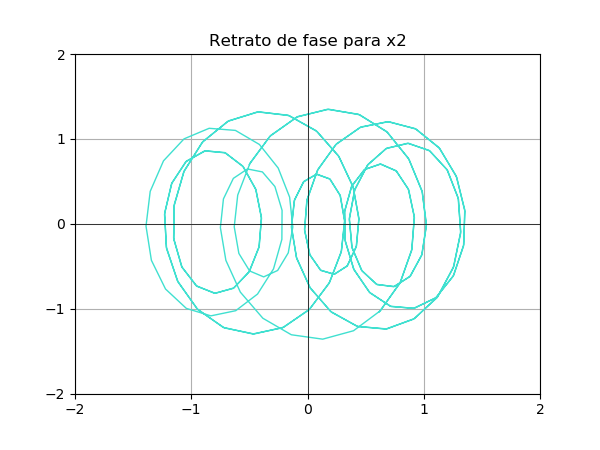
\includegraphics[width=.8\linewidth]{Ej2_32.png}
  \caption{Retrato de fase de $x_2$}
  \label{fig:sfig2}
\end{subfigure}
\begin{subfigure}{.55\textwidth}
  \centering
  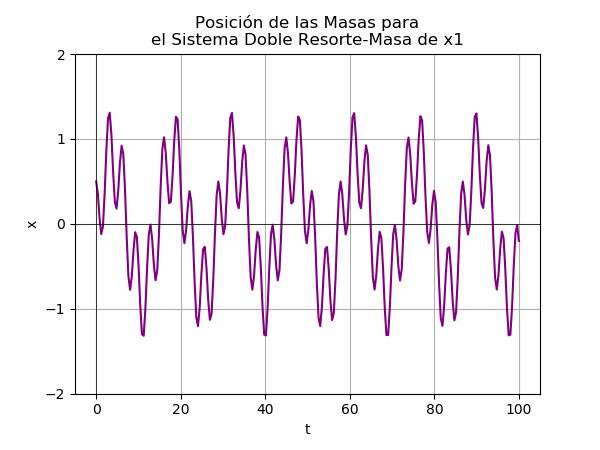
\includegraphics[width=.8\linewidth]{Ej2_33.png}
  \caption{Posición $x_1$ contra tiempo}
  \label{fig:sfig2}
\end{subfigure}
\begin{subfigure}{.55\textwidth}
  \centering
  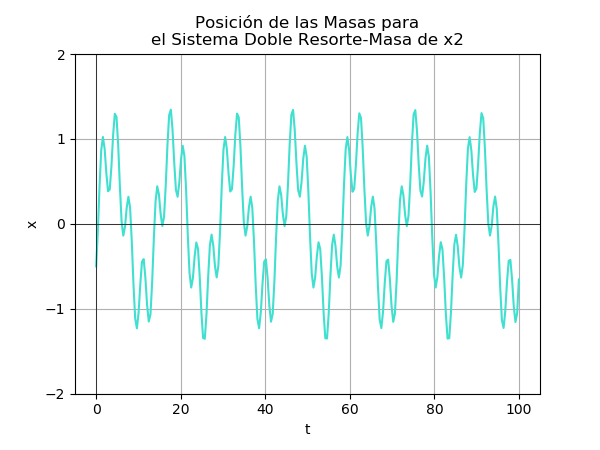
\includegraphics[width=.8\linewidth]{Ej2_34.png}
  \caption{Posición $x_2$ contra tiempo}
  \label{fig:sfig2}
\end{subfigure}
\begin{subfigure}{.55\textwidth}
  \centering
  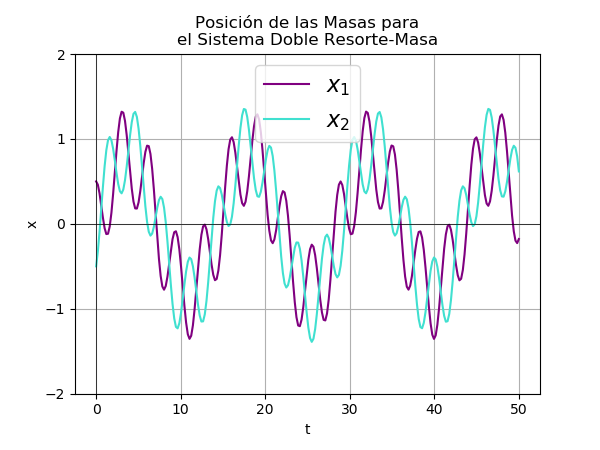
\includegraphics[width=.8\linewidth]{Ej2_35.png}
  \caption{Gráfica de $x_1$ y $x_2$}
  \label{fig:sfig2}
\end{subfigure}
\begin{subfigure}{.55\textwidth}
  \centering
  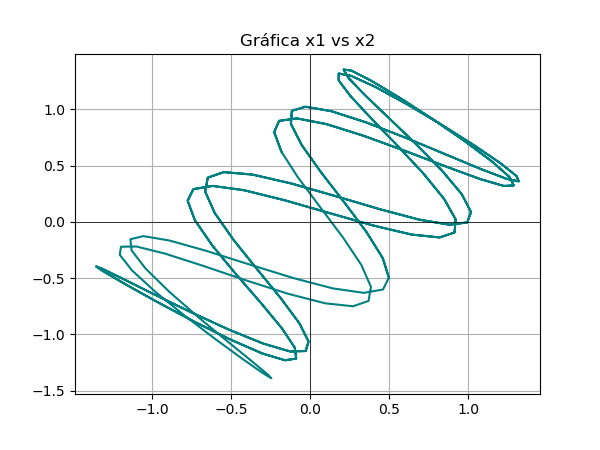
\includegraphics[width=.8\linewidth]{Ej2_36.png}
  \caption{Gráfica $x_1$ vs $x_2$}
  \label{fig:sfig2}
\end{subfigure}
\end{figure}

\subsection{Amortiguamiento}
Los problemas mas generales acerca de amortiguamiento es el de viscosidad, en donde la fuerza de amortiguamiento es proporcional a la velocidad. El amortiguamiento de la primera masa depende solamente de su velocidad y no en la de la segunda y viceversa. Si añadimos esta fuerza al modelo anteriormente descrito podemos obtener lo siguiente: \\

\centerline{$m_1 \ddot x_1 = -\delta \dot x_1 -k_1x_1 - k_2(x_1-x_2)$}
\centerline{$m_2 \ddot x_2 = -\delta \dot x_2 -k_2(x_2-x_1)$}
$    $

Se realiza el mismo proceso de obtener la ecuación de movimiento para una de las variables de posición, ya sea $x_1$ o $x_2$. Sustituimos esta ecuación en la anterior que le corresponde, y obtenemos de nuevo una ecuación diferencial lineal de cuarto grado para ambas posiciones de x. \\

\noindent \textit{2.4 Asume $m_1 = m_2 = 1$. Describe el movimiento para un sistema de resortes con $k_1=0.4$ y $k_2=1.808$, con coeficientes de amortiguamiento $\delta_1=0.1$ y $\delta_2=0.2$ con condiciones iniciales de $(x_1(0), \dot x_1(0), x_2(0), \dot x_2(0)$)=$(1,1/2,2,1/2)$.}\\

Como existe ahora un amortiguamiento, las amplitudes de ambos movimientos disminuyen conforme pasa el tiempo. Al graficar $x_1$ y $x_2$, podemos observar como se mueven casi en sincronía a pesar de que tienen distintas condiciones iniciales. El código para este caso es:  \\ 

\begin{figure}[h!]
    \centering
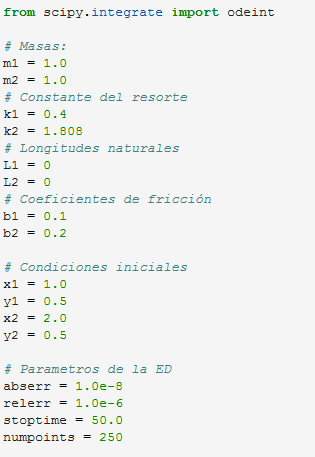
\includegraphics[width=2.5in]{Cod7.png}
\end{figure}

Las graficas resultantes fueron: \\ \\ \\
\begin{figure}[h!]
\begin{subfigure}{.55\textwidth}
  \centering
  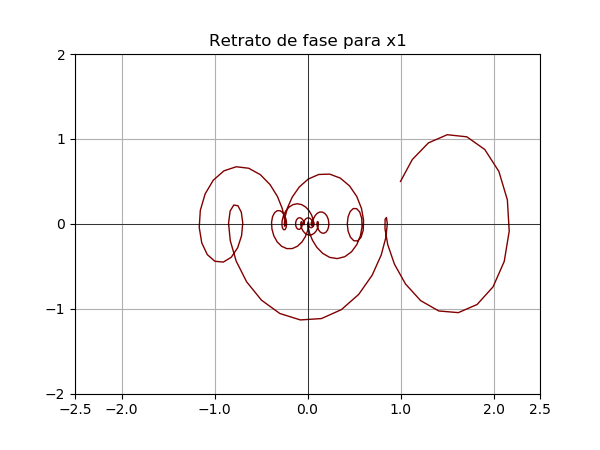
\includegraphics[width=.8\linewidth]{Ej2_41.png}
  \caption{Retrato de fase de $x_1$}
  \label{fig:sfig2}
\end{subfigure}
\begin{subfigure}{.55\textwidth}
  \centering
  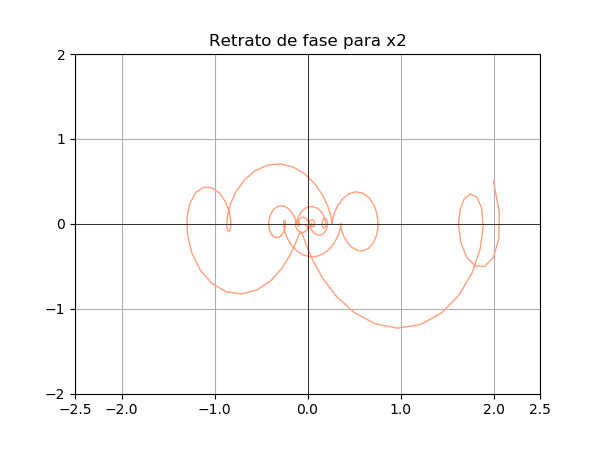
\includegraphics[width=.8\linewidth]{Ej2_42.png}
  \caption{Retrato de fase de $x_2$}
  \label{fig:sfig2}
\end{subfigure}
\begin{subfigure}{.55\textwidth}
  \centering
  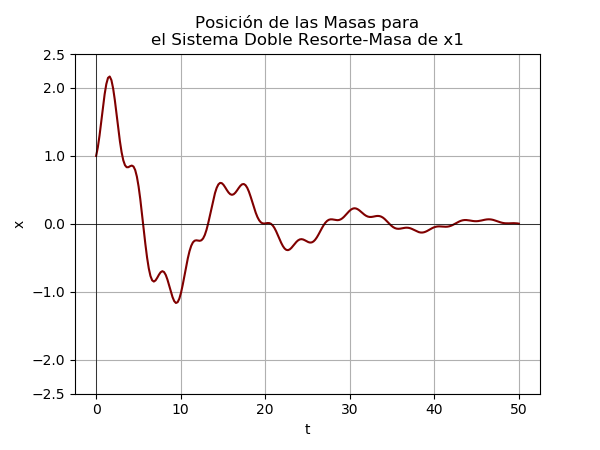
\includegraphics[width=.8\linewidth]{Ej2_43.png}
  \caption{Posición $x_1$ contra tiempo}
  \label{fig:sfig2}
\end{subfigure}
\begin{subfigure}{.55\textwidth}
  \centering
  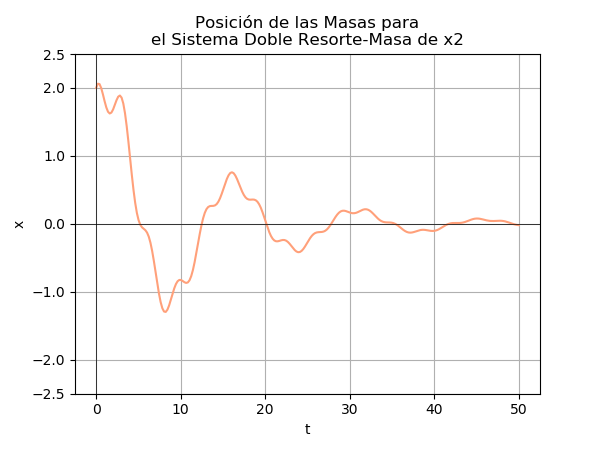
\includegraphics[width=.8\linewidth]{Ej2_44.png}
  \caption{Posición $x_2$ contra tiempo}
  \label{fig:sfig2}
\end{subfigure}
\begin{subfigure}{.55\textwidth}
  \centering
  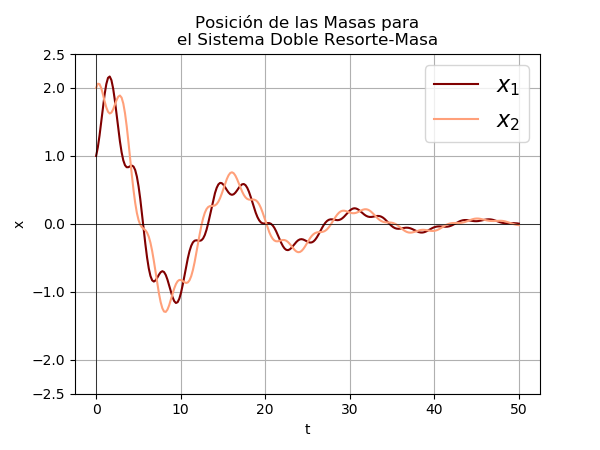
\includegraphics[width=.8\linewidth]{Ej2_45.png}
  \caption{Gráfica de $x_1$ y $x_2$}
  \label{fig:sfig2}
\end{subfigure}
\begin{subfigure}{.55\textwidth}
  \centering
  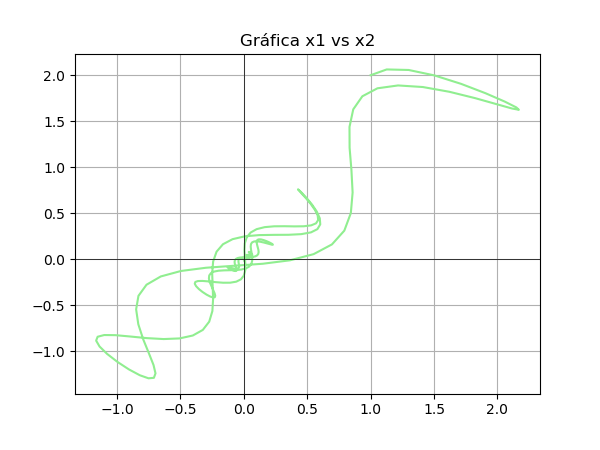
\includegraphics[width=.8\linewidth]{Ej2_46.png}
  \caption{Gráfica $x_1$ vs $x_2$}
  \label{fig:sfig2}
\end{subfigure}
\end{figure}

\section{Resultado analítico y resultado numérico}
Como en Python se realizo una aproximación numérica con los datos disponibles, y en el artículo se proporciona la solución analítica, es posible calcular el error relativo que hay entre nuestra aproximación y el valor real. Para hacer esto, en los primeros dos ejercicios, se imprimió en el archivo la definición del error relativo, restando el valor real al aproximado dividiendo esto entre el valor real. \\

Para el primer caso se obtuvo el error relativo calculando:

\begin{verbatim}
np.abs((w1[0]-(np.cos(np.sqrt(2.0)*t1)))/(np.cos(np.sqrt(2.0)*t1))) \\
np.abs((w1[2]-(2.0*np.cos(np.sqrt(2.0)*t1)))/(2.0*np.cos(np.sqrt(2)*t1)))
\end{verbatim}

En donde el primer comando es para $x_1$ y el segundo para $x_2$. Las graficas obtenidas del error relativo contra el tiempo, para el ejemplo 2.1 fueron:

\begin{figure}[h!]
\begin{subfigure}{.6\textwidth}
  \centering
  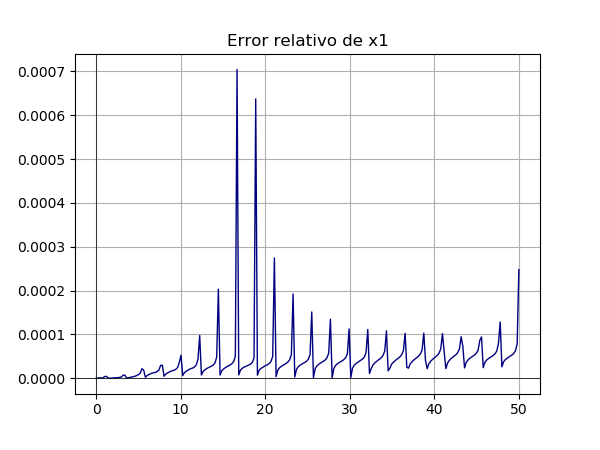
\includegraphics[width=.8\linewidth]{Ej2_14.png}
  \caption{Gráfica del error $x_1$ contra tiempo}
  \label{fig:sfig2}
\end{subfigure}
\begin{subfigure}{.6\textwidth}
  \centering
  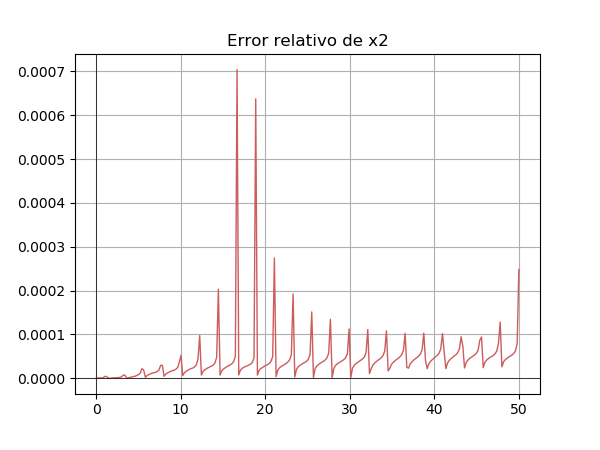
\includegraphics[width=.8\linewidth]{Ej2_15.png}
  \caption{Gráfica del error $x_2$ contra tiempo}
  \label{fig:sfig2}
\end{subfigure}
\end{figure}

Como se puede notar, los errores son muy pequeños, del orden de $7*10^{-3}$, y los errores entre $x_1$ y $x_2$ son idénticos. Este es el caso también para el ejemplo 2.2, donde el error es muy pequeño y casi igual para $x_1$ y $x_2$:

\begin{figure}[h!]
\begin{subfigure}{.6\textwidth}
  \centering
  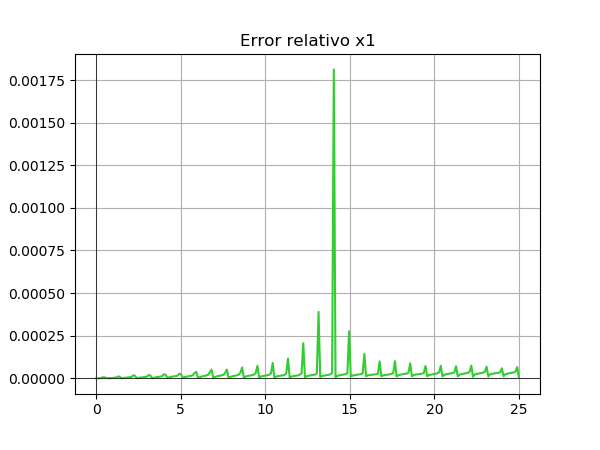
\includegraphics[width=.6\linewidth]{Ej2_23.png}
  \caption{Gráfica del error $x_1$ contra tiempo}
  \label{fig:sfig2}
\end{subfigure}
\begin{subfigure}{.6\textwidth}
  \centering
  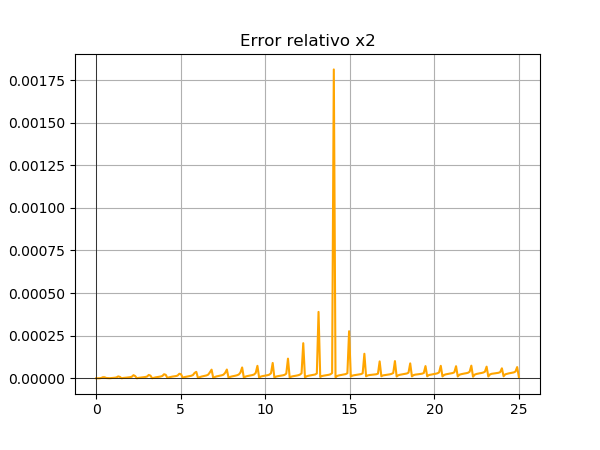
\includegraphics[width=.6\linewidth]{Ej2_24.png}
  \caption{Gráfica del error $x_2$ contra tiempo}
  \label{fig:sfig2}
\end{subfigure}
\end{figure}

\section{Conclusiones}
Este nuevo lugar de trabajo, Jupyter Lab, es mucho mas limpio y eficiente que el notebook. Este permite realizar cálculos y operaciones de una manera mas rápida y eficiente, esto gracias al uso de la librería scipy.integrate.odeint, que permite hasta resolver ecuaciones diferenciales. \\

Es muy interesante el poder que tiene el lenguaje Python, sin mencionar su habilidad para poder leer archivos y tomarlos como datos numéricos sin especificarlo. Cabe mencionar que el tema de esta actividad fue muy interesante, ya que el semestre anterior se cursó la clase de Mecánica II, en donde se vio este fenómeno de resortes acoplados, pero con este repaso tanto teórico como analítico queda mucho más claro como funciona este fenómeno. 

\section{Bibliografía}
\begin{itemize}
    \item Temple H. Fay, Sarah Duncan Graham (2003) Coupled Spring Equations. Int. J. Educ. Math. Sci. Tech.. Vol. 34, No. 1, pp. 65-79. Recuperado de: http://math.oregonstate.edu/~gibsonn/Teaching/MTH323-010S15 \\ /Supplements/coupled\_spring.pdf
    \item Oscilaciones amortiguadas. (2010) Recuperado de:http://www.sc.ehu.es/sbweb/fisica/oscilaciones \\ /amortiguadas/amortiguadas.htm
\end{itemize}

Imagenes utilizadas:
\begin{itemize}
    \item http://srv2.fis.puc.cl/mediawiki/index.php/Osciladores\_Acoplados\_(Fiz0312)
\end{itemize}
\section{Apéndice}
\noindent\textbf {1. ¿En general te pareció interesante esta actividad de modelación matemática? ¿Qué te gustó mas? ¿Qué no te gustó?} \\

Me gusto mucho esta actividad, este tema es uno de los que mas me gusto en Mecánica II, y poder repasarlo ahora con programación es muy interesante y divertido. Me gusto mucho las gráficas generadas por Python, sobre todo los retratos de fase, pero me hubiera gustado otras referencias acerca del tema. \\

\noindent\textbf {2. La cantidad de material te pareció ¿bien?, ¿suficiente?, ¿demasiado?}\\

La cantidad de material al principio me parecio que era mucha, sobre todo con el cambio de Jupyter Notebook a Lab, pero una vez empezando la práctica me di cuenta de que no era mucho problema. La cantidad es suficiente. \\ \\

\noindent\textbf {3. ¿Cuál es tu primera impresión de Jupyter Lab?  } \\

Me gusto mucho más que Jupyter Notebook, tiene un diseño que me parece mejor  y mas fácil de entender. Sin mencionar que las librerías y funciones que se pueden utilizar ahí son muy buenas e interesantes. \\

\noindent\textbf {4. Respecto al uso de funciones de SciPy, ¿ya habías visto integración numérica en tus cursos anteriores? ¿Cuál es tu experiencia?.} \\

En Análisis Numérico ya habíamos visto dos tipos de integración numérica, pero no de esta manera. Se utilizaron los métodos del trapecio y de Simpson, con un programa en Fortran, por lo cual este modo de integración es algo nuevo para mi. \\

\noindent\textbf {5. El tema de sistema de masas acopladas con resortes, ¿ya lo habías resuelto en tu curso de Mecánica 2?}\\

Si se había resuelto anteriormente, pero no con tantas especificaciones. Se vio de una manera rápida y sencilla, ya que en ese momento apenas estaba llevando ecuaciones diferenciales. \\

\noindent\textbf {6. ¿Qué le quitarías o agregarías a esta actividad para hacerla más interesante y divertida? }\\

Siento que esta práctica ya es buena como es, solamente me gustaría que tuviera mas referencias referente al tema para tener un mejor contexto y sea mas fácil de comprender.
\end{document}